% !TeX spellcheck = de_DE
\documentclass[]{article}

\usepackage[utf8]{inputenc}
\usepackage[T1]{fontenc}
\usepackage[scaled]{beramono}
\usepackage{amssymb}
\usepackage{amsmath}
\usepackage{graphicx}
\usepackage[top=2cm, bottom=2cm, left=2cm, right=4cm]{geometry}
\usepackage{csquotes}
\usepackage{listings}
\usepackage{hyperref}
\usepackage{booktabs}

\lstset{
	tabsize=2,
	language=Java,
	showstringspaces=false,
	basicstyle=\footnotesize\ttfamily,
}

%no indentation
\setlength\parindent{0pt}

\pagestyle{empty}

\begin{document}
	
	\section{Grammatiken}
	
	\begin{enumerate}
		\item Welche der Zeichenketten sind gültig bezüglich des abgebildeten Syntaxdiagramms?
		
		\begin{minipage}{0.4\linewidth}
		\begin{itemize}
			\item[$\square$] X
			\item[$\square$] XX
			\item[$\square$] XXXX
			\item[$\square$] XXXXX
			\item[$\square$] XXXXXXX
		\end{itemize}
		\end{minipage}
		\begin{minipage}{0.5\linewidth}
			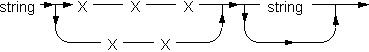
\includegraphics[width=\linewidth]{figures/syntax-string.png}
		\end{minipage}
		\vspace{2ex}
		
		\item Welche der Zeichenketten sind gültig bezüglich des abgebildeten Syntaxdiagramms?
		
		\begin{minipage}{0.4\linewidth}
			\begin{itemize}
				\item[$\square$] 212
				\item[$\square$] 333
				\item[$\square$] 22394
				\item[$\square$] 0330
				\item[$\square$] 6135798
			\end{itemize}
		\end{minipage}
		\begin{minipage}{0.5\linewidth}
			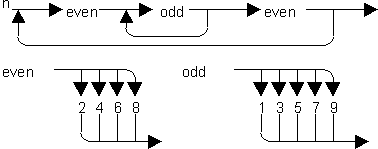
\includegraphics[width=\linewidth]{figures/syntax-evenodd.png}
		\end{minipage}
		\vspace{2ex}
		
		\item Überführen Sie die folgende Grammatik in EBNF in äquivalente Syntaxdiagramme:
		
		\texttt{digitWithoutZero ::= '1' | '2' | '3' | '4' | '5' | '6' | '7' | '8' | '9'\\[1ex]
		digit ::= '0' | digitWithoutZero	\\[1ex]
		nat ::= digitWithoutZero \{digit\}\\[1ex]
		integer ::= ['-'] nat}
		
		\vspace{30ex}
	
		\item Beschreiben Sie die Bildung von deutschen Zahlwörtern bis 9999 als EBNF.\\ Beispiel: Fünftausendsiebenhundertsechsunddreißig.
		
	\end{enumerate}
	
	\newpage
	
	\section{Struktogramme}

	Geben Sie zu dem folgenden C-Segment ein äquivalentes Struktogramm an.
	
	\begin{lstlisting}[gobble=4]
		int sum, num;
		sum = 0;
		scanf("%d", &num);
		while (num > 0) {
			sum = sum + (num % 10);
			num = num / 10;
		}
		printf("%d\n", sum);
	\end{lstlisting}
	
	\vspace{30ex}
	
	\section{Programmieren}
	
	Schreiben Sie ein Programm, das eine Temperatur in Grad Celsius einliest, dann in Fahrenheit umrechnet und beide Temperaturen ausgibt.
	Recherchieren Sie selbständig die Umrechnungsformel.\\
	\textit{Bonus: Das Ergebnis soll mit genau einer Nachkommastelle ausgegeben werden.}
	
\end{document}